\section{The need for fine-granularity streams (existing techniques)}
Here we argue that streaming by bit planes or streaming by levels result in sub-optimal PSNR (figure \ref{fig:psnr_traditional_vs_by_norm_viscosity})

\begin{figure}[t]
	\centering
	\subcaptionbox{without skip leading zeros}
	{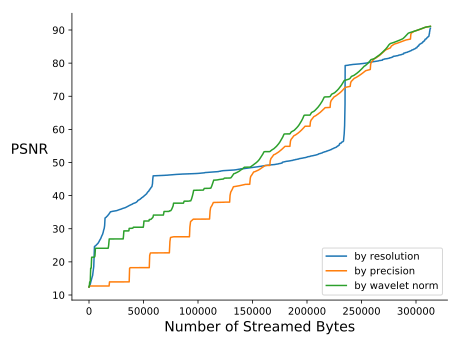
\includegraphics[width=0.4\linewidth]{resources/rmse-miranda-viscosity.png}}
	\subcaptionbox{with skip leading zeros}
	{\includegraphics[width=0.4\linewidth]{resources/rmse-miranda-viscosity_slz.png}}
	\caption {PSNR comparison between three streams: by bit-plane, by level, and by wavelet norm}
	\label{fig:file_zero}
\end{figure}

When compression is used, it avoids streaming the leading zero bits of the wavelet coefficients.

We compare data-independent streams. Figure 1: PSNR comparison for a data set (Miranda viscosity?)
\begin{enumerate}
  \item Data-independent, by-bit-plane stream (truncation stream)
  \item Data-independent, by-level stream (idx style, mipmap)
  \item Data-independent, by-bit-importance stream
\end{enumerate}

Datasets:
\begin{enumerate}
  \item Miranda viscosity (smooth and uniform)
  \item Kingsnake (noisy and sparse)
  \item Magnetic (tiny narrow lines)
  \item Euler 2D (sharp front)
  \item Enzo u (wide range)
\end{enumerate}

\section{Data-dependent streams}

\begin{enumerate}
  \item First we compare data-dependent streams. Figure 2: PSNR comparison for the same data set
  \begin{enumerate}
    \item Data-dependent, by-bit-plane stream with constraints on bit plane ordering
    \item Data-dependent, by-level stream with constraints on bit plane ordering
    \item Data-dependent stream with constraints on bit plane ordering
    \item Data-dependent, by-bit-plane stream with skip leading zeros
    \item Data-dependent, by-level stream with skip leading zeros
    \item Data-dependent stream with skip leading zeros
  \end{enumerate}

  \item The reader may ask: if I already have a good, practical PSNR stream (the data-independent, by bit plane, skip leading zeros), why do I need other streams? Here we show that for isocontour extraction, and for histogram computation, we are better off with other streams.
  
  Figure 3: isocontour error for the same data set
    \begin{enumerate}
      \item Data-independent, by-bit-plane, normalized, skip leading zeros
      \item Data-dependent stream for RMSE with skip leading zeros
      \item Data-dependent stream for isocontour with skip leading zeros
    \end{enumerate}
  We also need to show a rendering of the isocontour for all three streams at some low bit rate.
  Figure 4: histogram error for the same data set
    \begin{enumerate}
      \item Data-independent, by-bit-plane, normalized, skip leading zeros
      \item Data-dependent stream for RMSE with skip leading zeros
      \item Data-dependent stream for isocontour with skip leading zeros
  \end{enumerate}  
  Here we also show renderings of different histograms corresponding to the different streams at some low bit rate.
\end{enumerate}
